\section{Two-Body Green's Function\label{sect:ppRPA}}
In the same way the one-hole spectral function (\ref{eq:defS}) gives 
information on the one-body removal reaction, the two-hole spectral
function contains 
information about what two nucleons are doing inside the nucleus. The formulas 
in this section are derived in an analogous way as the formulas in the 
previous sections.
First, the two-body spectral function is defined as
%
	\begin{equation}
		S^{hh}_{\alpha\beta\gamma\delta}(\omega)
	=
		-\frac{1}{\pi} 
		\; 
		{\rm Im}
		\; 
		G^{II}_{\alpha\beta\gamma\delta}(\omega)
	\;,
	\end{equation}
%
with $G^{II}(\omega)$ the Fourier transform (Lehmann representation) of
%
	\begin{equation}
		iG^{II}_{\alpha\beta\gamma\delta} (t-t') 
	=
		\ME< \Psi^A_0 | 
		T \left[
		\Oa{\beta} (t) \Oa{\alpha}(t)
		\Oc{\gamma}(t')\Oc{\delta}(t')
		\right]
		|\Psi^A_0 >
	\label{eq:g2t}
	\;.
	\end{equation}
%

\subsection{The Bethe-Salpeter Equation for $G^{II}$\label{sec:lrcBSE}}
When the single-particle basis and the Hamiltonian are specified, one can 
derive an equation for the two-particle Green's function 
(\ref{eq:g2t}). 
%
With the Hamiltonian (\ref{eq:Hamiltonian}) 
a Feynman-Dyson expansion for the general two-particle Green's function with
four time arguments (\ref{eq:g2t}) 
can be derived from the theorem of Gell-Mann and Low\cite{FW71,AGD63}
%
	\begin{eqnarray}
	\lefteqn{%
		iG^{II}_{\alpha\beta\gamma\delta}
		         (t_1, t_2, t_3, t_4) 
	=
		\ME< \Psi^A_0 | 
		T \left[
		\Oa{\beta}(t_2) \Oa{\alpha}(t_1)
		\Oc{\gamma}(t_3) \Oc{\delta}(t_4)
		\right]
		|\Psi^A_0 >
	} && 
	\label{eq:GMLG} \\
	&=&
		\sum_{m=0}^{\infty}
		\frac{(-i)^m}{m!}
 		\int\limits_{-\infty}^{\infty} 
		{\rm d} t'_1 \cdots {\rm d} t'_m
	\nonumber\\
	&&
		\inp< \Phi_0 | 
			T\left[
				H_1(t'_1)\cdots H_1(t'_m)
				\Oa{\beta}(t_2) \Oa{\alpha}(t_1)
				\Oc{\gamma}(t_3) \Oc{\delta}(t_4)
			 \right]
		    | \Phi_0 >_c 
	\nonumber
	\;,
	\end{eqnarray}
%
where the subscript $c$ means that only the `connected' terms should
be taken into account only.
This expansion can be written in the form of  the 
Bethe-Salpeter equation (BSE) 
%
	\begin{eqnarray}
	\lefteqn{%
		G^{II}_{\alpha\beta\gamma\delta}
		         (t_1, t_2, t_3, t_4) 
	=} && \label{eq:BSEpp} \\
	&&
	i\left[
		g_{\alpha\gamma}(t_1-t_3)
		g_{\beta\delta}(t_2-t_4)
	-
		g_{\alpha\delta}(t_1-t_4)
		g_{\beta\gamma}(t_2-t_3)
	\right]
	\nonumber \\
	&&
	-
 		\int\limits_{-\infty}^{\infty} 
		{\rm d} t'_1 {\rm d} t'_2 {\rm d} t'_3 {\rm d} t'_4
		\sum_{\mu\nu\kappa\lambda}
	\nonumber \\
	&&
	\left[
		g_{\alpha\mu}(t_1-t'_1)
		g_{\beta\nu}(t_2-t'_2)
	\right]
		\Gamma^{pp}_{\mu\nu\kappa\lambda}
		(t'_1, t'_2, t'_3, t'_4)
		G^{II}_{\kappa\lambda\gamma\delta}
		(t'_3, t'_4, t_3, t_4) 
	\nonumber
	\;.
	\end{eqnarray}
%
The particle-particle vertex $\Gamma^{pp}$ should be particle-particle 
irreducible to avoid double-counting\cite{Mi67}.
The single-particle Green's functions $g$ are solutions to the 
Dyson equation (\ref{eq:Dyson}).
A graphical representation of the BSE (\ref{eq:BSEpp}) is given in
in fig.~\ref{fig:BSEpp}.
%%%%%%%%%%%%%%
\begin{figure}
\centerline{
\epsfig{ file=figures/BSEpp.eps, height=4cm }
}
\caption[]{Graphical representation of the Bethe-Salpeter equation 
(\ref{eq:BSEpp}). Time runs vertically.
A double line indicate a `dressed' single-particle propagator $g$. The 
boxes with $G^{II}$ are the two-particle Green's functions. The box with
$\Gamma^{pp}$ denotes the particle-particle vertex, dependent on four
times.
\label{fig:BSEpp}
}
\end{figure}
%%%%%%%%%%%%%%

The two-particle Green's function (\ref{eq:g2t}) is connected to the 
two-particle Green's function in (\ref{eq:BSEpp}) by the limit 
 $t_1 \rightarrow t_2$, $t_3 \rightarrow t_4$. When the 
restriction $t'_3=t'_4$ is imposed on the two-particle vertex
 $\Gamma^{pp}$, (\ref{eq:BSEpp}) reduces to an equation for the two-times
Green's function (\ref{eq:g2t}). 

\subsection{Approximations to the BSE}
In the expansion for $\Gamma^{pp}$ the
first term will be $\hat{H}_1$. 
The approximation $\Gamma=\hat{H}_1$ simplifies the BSE 
dramatically when $\hat{H}_1$ is a static two-body interaction (no retardation).
With this assumption, the Green's function $G^{II}$  will only
depend on two times
%
	\begin{eqnarray}
	\lefteqn{%
		G^{II}_{\alpha\beta\gamma\delta}
		         (t_1, t_2) 
	=} && \label{eq:BSEHpp} \\
	&&
	i\left[
		g_{\alpha\gamma}(t_1-t_2)
		g_{\beta\delta}(t_1-t_2)
	-
		g_{\alpha\delta}(t_1-t_2)
		g_{\beta\gamma}(t_1-t_2)
	\right]
	\nonumber \\
	&-&
		\sum_{\mu\nu\kappa\lambda}
 		\int\limits_{-\infty}^{\infty} 
		{\rm d} t_3 
	\left[
		g_{\alpha\mu}(t_1-t_3)
		g_{\beta\nu}(t_1-t_3)
	\right]
		V_{\mu\nu\kappa\lambda}
		G^{II}_{\kappa\lambda\gamma\delta}
		(t_3, t_2) 
	\nonumber
	\;.
	\end{eqnarray}
%
This equation represents  all the ladder diagrams. It thereby sums a similar
class of diagrams within the model space as summed by the Bethe-Goldstone
equation for (intermediate) configurations outside the model space.
Within the model space, \ie\ for low (relative) momenta, the interaction is 
attractive, however. It may then give rise to the formation of collective pair 
structure of \eg\ BCS type\cite{BCS57}. The RPA may then be thought to describe 
`pairing vibrations'\cite{BHR73,RS80}, \ie\ formation of pairs in a 
`pairing field' and exchanges with a projectile nucleus which acts as a 
reservoir.

The equation (\ref{eq:BSEHpp}) can be solved in Fourier transformed 
form by the same methods as
for the particle-hole DRPA, once the one-body Green's functions $g$ are known. 
%
Using the form (\ref{eq:g1s}) for the single-particle Green's function (\ie\
using the definitions (\ref{eq:defsSE}))
the Fourier transform of the inhomogeneous term of (\ref{eq:BSEHpp}) (the term 
that does not contain the residual interaction explicitly) can
be written as 
%
	\begin{eqnarray}
	\lefteqn{%
		G^{II,f}_{\alpha\beta\gamma\delta}(\omega)
	=
		\left[
			\delta_{\alpha\gamma}
			\delta_{\beta\delta}
		-
			\delta_{\alpha\delta}
			\delta_{\beta\gamma}
		\right]
		\int
		\frac{{\rm d} \omega'}
		     { 2 \pi }
		\;
		g_{\alpha}(\omega)
		g_{\beta}(\omega-\omega')
	}
	\label{eq:G2f} \\
	&=&
		\left[
			\delta_{\alpha\gamma}
			\delta_{\beta\delta}
		-
			\delta_{\alpha\delta}
			\delta_{\beta\gamma}
		\right]
	\nonumber \\
	& \times&
		\left[
		\sum_{ij}
		\frac{
		S^p_{\alpha,i} S^p_{\beta,j}
		}{ \omega - E^p_{\alpha,i} - E^p_{\beta,j} + i \eta }
	-
		\sum_{kl}
		\frac{
		S^h_{\alpha,k} S^h_{\beta,l}
		}{ \omega - E^h_{\alpha,k} - E^h_{\beta,l}- i \eta }
		\right]
	\nonumber 
	\end{eqnarray}
%
The input of a single-particle propagator from a certain calculation leads
straightforwardly to a first approximation for the two-particle propagator
($G^{II} = G^{II,f}$). Even the following step, analogous to phDRPA, is 
computationally not very expensive. 

The two-proton Green's function, as given in
(\ref{eq:BSEpp}), will be used in chapter~\ref{chap:ppknock}
to describe the shell model structure of the reaction amplitudes. 
In order to obtain the high-momentum components of the two-nucleon spectral 
function, this structure is there supplemented with defect functions obtained 
from the Bethe-Goldstone equation in a consistent way.
